%!TEX ROOT=formularioFisica.tex

\section{Fluidodinamica}\label{sec:idrodinamica}
L'idrodinamica studia i movimenti dei liquidi e la loro relazione con il contenitore.\\
Il seguete disegno verrà utilizzato per definire le formule e far capire il significato delle 
lettere.\\
Per gli esercizi, si vada a pagina~\pageref{ex:idrodinamica}.
\begin{center}
  \begin{tikzpicture}[scale=0.6]
    % Coordinates for bottom curve
    \coordinate (BottomLeft) at (-5,0);
    \coordinate (BottomJunct1) at (-1, 0);
    \coordinate (BottomJunct2) at (1, 0.8);
    \coordinate (BottomRight) at (5, 0.8);
    % Coordinates for top curve
    \coordinate (TopLeft) at ($(BottomLeft) + (0,1)$);
    \coordinate (TopJunct1) at ($(BottomJunct1) + (0,1)$);
    \coordinate (TopJunct2) at ($(BottomJunct2) + (0,1.3)$);
    \coordinate (TopRight) at ($(BottomRight) + (0,1.3)$);
    % Defines the 2 radiuses for the circles and cilinders
    \def\Rs{0.5};
    \def\RB{0.65};
    % Define the centers of the circles for the cilinders
    \coordinate (BottomCircL) at (-4, \Rs);
    \coordinate (BottomCircR) at (-2.5, \Rs);
    \coordinate (TopCircL) at (2.5, 0.8+\RB);
    \coordinate (TopCircR) at (4, 0.8+\RB);

    % Draws the bottom line
    \draw (-6, -1) -- (6, -1);
    % Draws the pipe
    \draw (BottomLeft) -- (BottomJunct1) to[out=0, in=180] (BottomJunct2) -- (BottomRight);
    \draw (TopLeft) -- (TopJunct1) to[out=0, in=180] (TopJunct2) -- (TopRight);
    % Draws the ellipses
    \filldraw[cyan!40] (BottomCircL) ellipse (0.1 and \Rs);
    \draw[dashed, cyan] (BottomCircR) ellipse (0.1 and \Rs);
    \filldraw[cyan!40] (TopCircL) ellipse (0.1 and \RB);
    \draw[dashed, cyan] (TopCircR) ellipse (0.1 and \RB);
    % Draws the comments
    % h_1
    \draw[|<->|, red] ($(BottomCircL) + (1, 0)$) -- ++(0, -1.5)
      node[pos=0.5, right]{$h_1$};
    % h_2
    \draw[|<->|, red] ($(TopCircL) + (1, 0)$) -- ++(0, -2.45)
      node[pos=0.5, left]{$h_2$};
    % A_1
    \node[cyan] (A1) at ($(BottomCircL) + (-0.5, -1)$) {$A_1$};
    \draw[-stealth, cyan] ($(BottomCircL)$) to[out=180, in=90] (A1);
    % A_2
    \node[cyan] (A2) at ($(TopCircL) + (-0.5, -1)$) {$A_2$};
    \draw[-stealth, cyan] ($(TopCircL)$) to[out=180, in=90] (A2);
    % L_1
    \draw[|<->|, blue] ($(BottomCircL) + (0, 0.7)$) -- ($(BottomCircR) + (0, 0.7)$)
      node[pos=0.5, above]{$\mathcolor{olive}{v_1}\Delta t = l_1$};
    % L_2
    \draw[|<->|, blue] ($(TopCircL) + (0, 0.9)$) -- ($(TopCircR) + (0, 0.9)$)
      node[pos=0.5, above]{$\mathcolor{olive}{v_2}\Delta t = l_2$};
    % P_1
    \draw[-latex, double, olive] ($(BottomCircL) + (-0.8, 0)$) -- ++(0.8, 0)
    node[pos=0, left] {$p_1$};
    % P_2
    \draw[-latex, double, olive] ($(TopCircL) + (-0.8, 0)$) -- ++(0.8, 0)
    node[pos=0, left] {$p_2$};
    % P_1
    \draw[-latex, double, orange] (BottomCircR) -- ++(0.8, 0)
    node[pos=1, right] {$v_1$};
    % P_2
    \draw[-latex, double, orange] (TopCircR) -- ++(0.8, 0)
    node[pos=1, right] {$v_2$};
  \end{tikzpicture}
\end{center}
\subsection{Equazione di Bernoulli}
Quest'equazione descrive un qualsiasi moto tra due punti di un qualsiasi fluido.
\begin{equation*}
  \mathcolor{olive}{p_1} + \delta g\mathcolor{red}{h_1} +
  \frac{1}{2}\delta\mathcolor{orange}{v_1}^2 = 
  \mathcolor{olive}{p_2} + \delta g\mathcolor{red}{h_2} +
  \frac{1}{2}\delta\mathcolor{orange}{v_2}^2
\end{equation*}
\hyperref[tab:g]{$g$}: $9.81\,\text{m/s}^2$\\
$\delta$: densità del fluido

\subsection{Attrito nei fluidi}
Un corpo che si muove in un fluido è rallentato da una forza di attrito. In particolare per una
sfera è pari a
\begin{equation*}
  F_a = \eta 6\pi rv
\end{equation*}
$\eta$: viscosità\\
$r$: raggio\\
$v$: velocità\\ [\baselineskip]
Tutti i corpi sferici che cadono hanno una velocità limite (in cui l'accelerazione è $0$) che si può
ricavare risolvendo
\begin{equation*}
  \eta6\pi rv_{\text{lim}}+\delta_{\text{fluido}}V_{\text{corpo}}g-mg=0
\end{equation*}

\begin{center}
  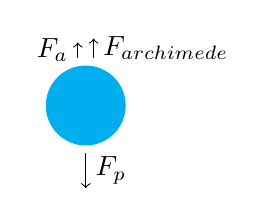
\begin{tikzpicture}[scale=0.5]
    \filldraw[cyan] (0,0) circle (1);
    \draw[->] (0,-1.2) -- ++(0,-0.9)
      node[pos=0.5,right]{$F_p$};
    \draw[->] (-0.2,1.2) -- ++(0,0.4)
      node[pos=0.5,left]{$F_a$};
    \draw[->] (0.2,1.2) -- ++(0,0.5)
      node[pos=0.5,right]{$F_{\text{archimede}}$};
  \end{tikzpicture}
\end{center}

\subsection{Portata}
La portata descrive quanto fluido attraversa una sezione nel tempo.
\begin{equation*}
  \text{Portata} = \frac{\Delta V}{\Delta t} 
\end{equation*}
\begin{equation*}
  A_1v_1=A_2v_2
\end{equation*}
$A$: area della sezione\\
$v$: velocità del fluido\\
$V$: volume

\subsection{Equazione di Torricelli}
Si usi questa formula quando si deve trovare a che velocità esce un liquido da un contenitore.
\begin{center}
  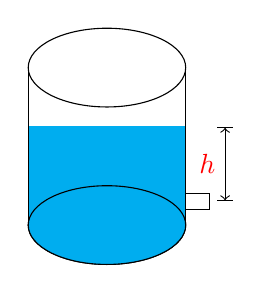
\begin{tikzpicture}
    \draw (0,0) ellipse (1 and 0.5);
    \draw (0,-2) ellipse (1 and 0.5);

    \filldraw[cyan] (-1,-0.75) -- (-1,-2) -- (1,-2) -- (1,-0.75) -- cycle;
    \filldraw[black, fill = cyan] (0,-2) ellipse (1 and 0.5);
    \draw (1,-1.8) -- ++(0,0.2) -- ++(0.3,0) -- ++(0,-0.2) -- cycle;
    \draw (-1,0) -- ++(0,-2);
    \draw (1,0) -- ++(0,-2);
    \draw[|<->|] (1.5,-1.7) -- (1.5,-0.75)
      node[red, pos=0.5, left]{$h$};
  \end{tikzpicture}
\end{center}
\begin{equation*}
  v = \sqrt{2g\mathcolor{red}{h}}
\end{equation*}
\hyperref[tab:g]{$g$}: $9.81\,\text{m/s}^2$\\
$\mathcolor{red}{h}$: altezza della colonna di fluido premente sul punto d'uscita
